\documentclass[11pt]{beamer}

\usepackage[english]{babel}
\usepackage[T1]{fontenc}
\usepackage[utf8]{inputenc}
\usepackage{mathtools}                       % matma
\usepackage{amsfonts,amsmath,amssymb,amsthm} % matma
\usepackage{listings}                        % załączanie kodu źródłowego
\usepackage{tikz}                            % rysowanie i grafy https://tikz.dev/tikz, https://centrality.mimuw.edu.pl/editor
\usepackage{pgf}
\usepackage{graphicx}

\title{Networkx Graph Visualization}
\author{Stanisław Bitner, Aleksander Wojsz}
\date{\today}

\usetheme{Warsaw}
\usecolortheme{orchid}

\setbeamertemplate{footline}[Warsaw]
\setbeamertemplate{headline}{}
\setbeamertemplate{page number in head/foot}[totalframenumber]
\setbeamertemplate{navigation symbols}{}

\usetikzlibrary{positioning,overlay-beamer-styles,graphs,fit,shapes}
\tikzset{}

\lstset{basicstyle=\ttfamily\footnotesize,keywordstyle=\color{magenta},tabsize=2,escapeinside=||,mathescape=true}

\AtBeginSection[] {
    \begin{frame}{\secname}
        \tableofcontents[currentsection,hideothersubsections,sectionstyle=hide]
    \end{frame}
}

\begin{document}

\frame{\titlepage}

\begin{frame}
    \frametitle{Table of contents}
    \tableofcontents[hideallsubsections]
\end{frame}

\section{Intro}

\subsection{Math Representation}
\begin{frame}{\subsecname}
    \begin{align*}
        G &= \left\langle V, E \right\rangle\\
        V &= \left\{ 1 \hdots 9 \right\}\\
        E &= \{\\
            &\{ 1, 2 \}, \{ 1, 3 \}, \{ 2, 4 \}, \{ 2, 5 \}, \{ 2, 6 \},\\
            &\{ 3, 5 \}, \{ 3, 6 \}, \{ 4, 7 \}, \{ 4, 8 \}, \{ 5, 7 \},\\
            &\{ 5, 8 \}, \{ 6, 7 \}, \{ 6, 8 \}, \{ 7, 9 \}, \{ 8, 9 \}\\
        \}
    \end{align*}
\end{frame}

\subsection{Hand Drawing}
\begin{frame}{\subsecname}
    \begin{figure}
        \centering
        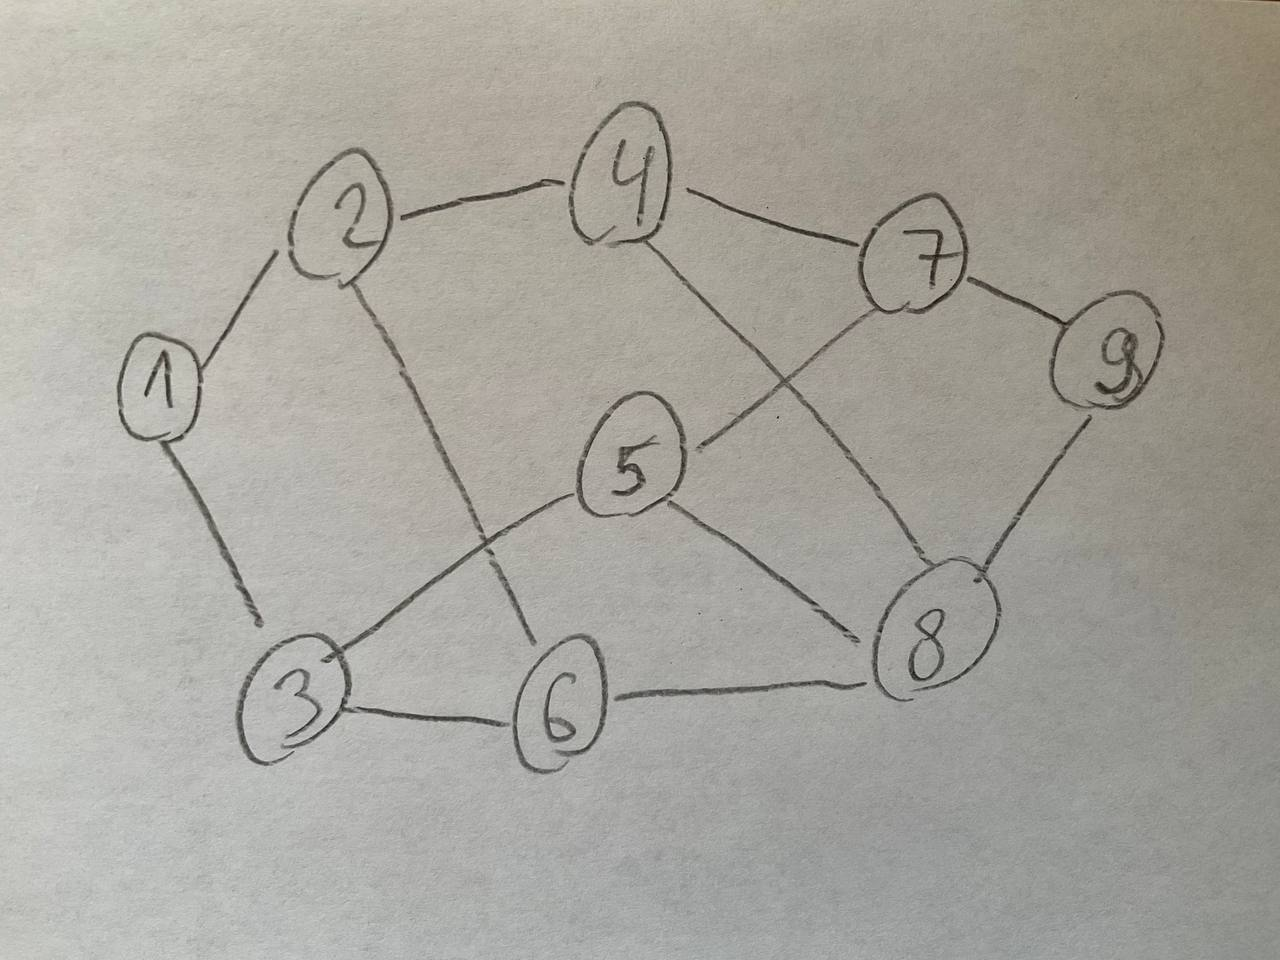
\includegraphics[width=0.8\textwidth]{figures/hand1.jpg}
    \end{figure}
\end{frame}

\begin{frame}{\subsecname}{Mistake}
    \begin{figure}
        \centering
        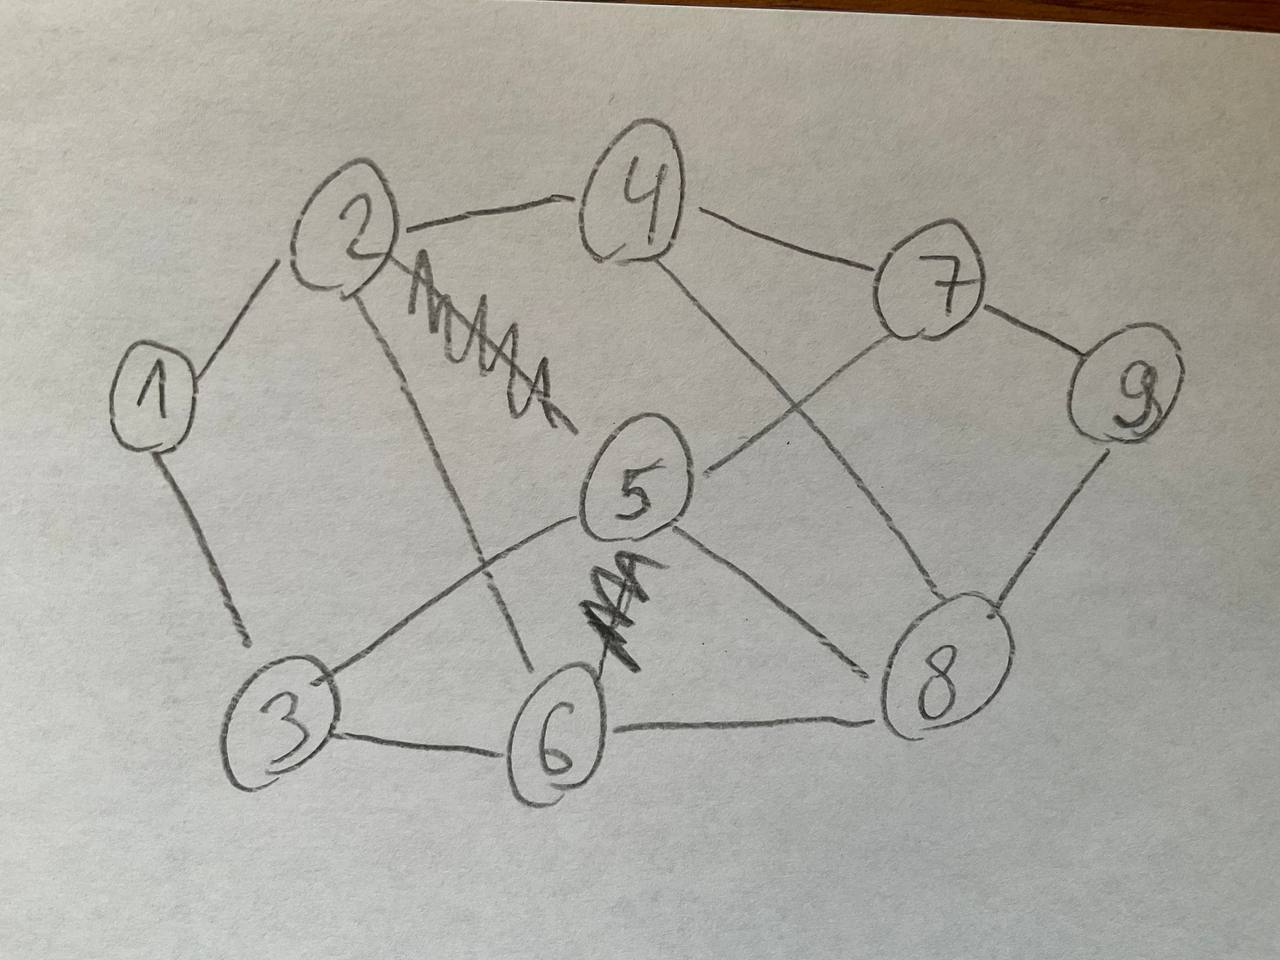
\includegraphics[width=0.8\textwidth]{figures/hand2.jpg}
    \end{figure}
\end{frame}

\begin{frame}{\subsecname}{Mistake}
    \begin{figure}
        \centering
        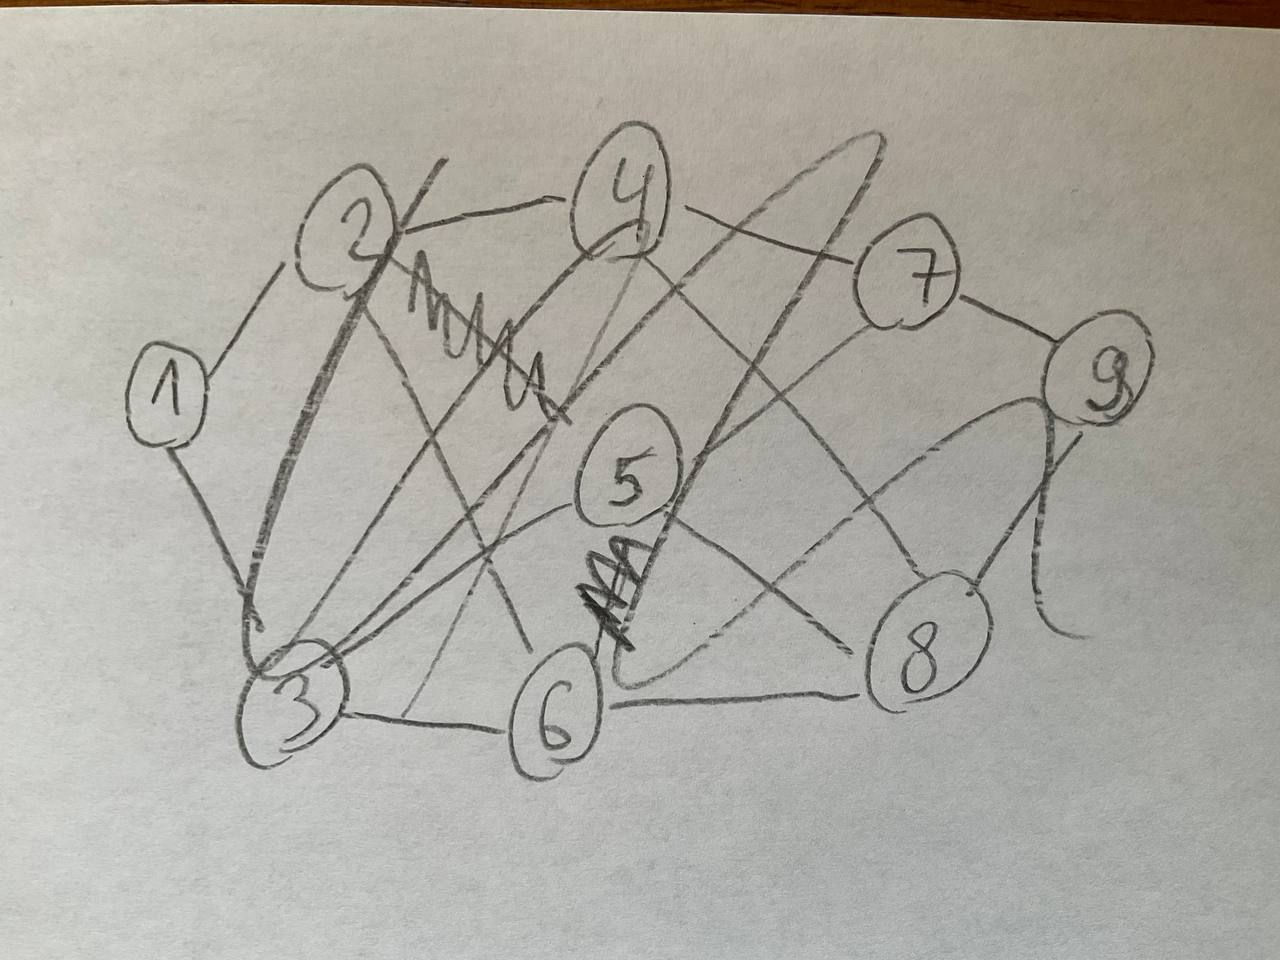
\includegraphics[width=0.8\textwidth]{figures/hand3.jpg}
    \end{figure}
\end{frame}

\subsection{Tablet Drawing}
\begin{frame}{\subsecname}
    \begin{figure}
        \centering
        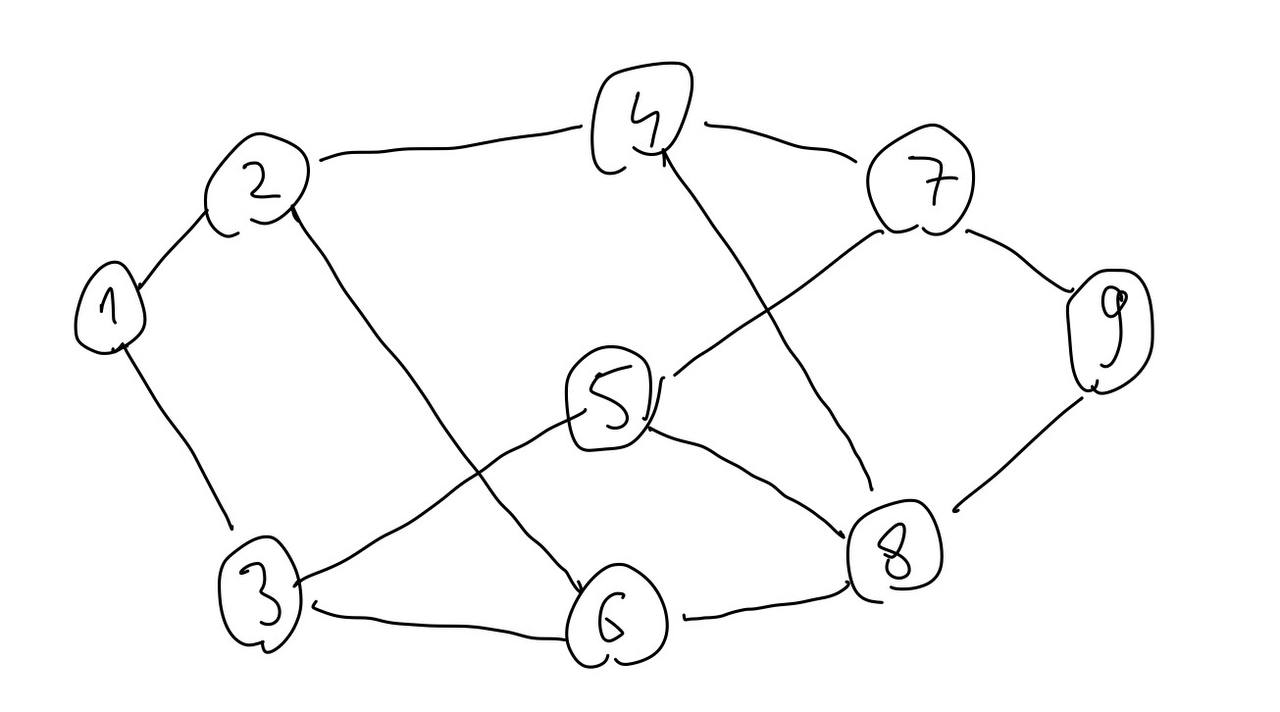
\includegraphics[width=0.8\textwidth]{figures/tablet.jpg}
    \end{figure}
\end{frame}

\subsection{Tikz}
\begin{frame}{\subsecname}
    \begin{figure}[h]
        \centering
        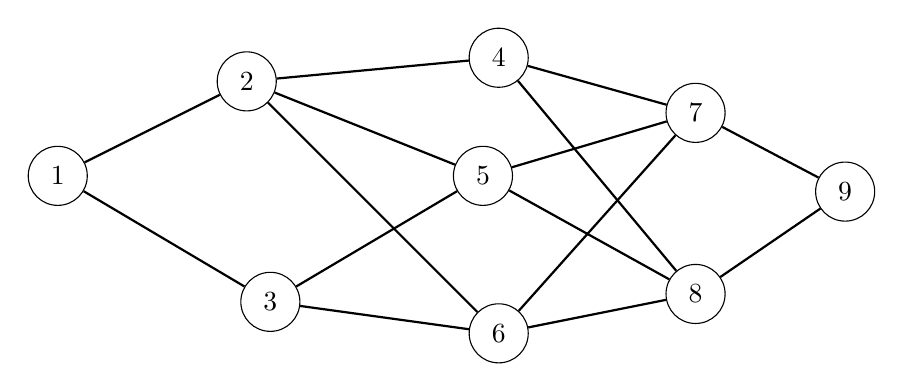
\begin{tikzpicture}[x=10cm,y=10cm]
            \tikzset{     
                e4c node/.style={circle,draw,minimum size=0.75cm,inner sep=0}, 
                e4c edge/.style={sloped,above,font=\footnotesize}
            }
            \node[e4c node] (1) at (0.00, 0.89) {1}; 
            \node[e4c node] (2) at (0.24, 1.01) {2}; 
            \node[e4c node] (3) at (0.27, 0.73) {3}; 
            \node[e4c node] (4) at (0.56, 1.04) {4}; 
            \node[e4c node] (5) at (0.54, 0.89) {5}; 
            \node[e4c node] (8) at (0.81, 0.74) {8}; 
            \node[e4c node] (7) at (0.81, 0.97) {7}; 
            \node[e4c node] (9) at (1.00, 0.87) {9}; 
            \node[e4c node] (6) at (0.56, 0.69) {6}; 
            \path[draw,thick]
                (1) edge[e4c edge]  (2)
                (1) edge[e4c edge]  (3)
                (2) edge[e4c edge]  (4)
                (2) edge[e4c edge]  (5)
                (2) edge[e4c edge]  (6)
                (3) edge[e4c edge]  (5)
                (3) edge[e4c edge]  (6)
                (4) edge[e4c edge]  (7)
                (4) edge[e4c edge]  (8)
                (5) edge[e4c edge]  (7)
                (5) edge[e4c edge]  (8)
                (6) edge[e4c edge]  (7)
                (6) edge[e4c edge]  (8)
                (7) edge[e4c edge]  (9)
                (8) edge[e4c edge]  (9)
                ;
        \end{tikzpicture}
    \end{figure}
\end{frame}

\begin{frame}[fragile]{\subsecname}{Code}
    \begin{block}{}
        \begin{lstlisting}[language=tex]
            \node[e4c node] (1) at (0.00, 0.89) {1}; 
            \node[e4c node] (2) at (0.24, 1.01) {2}; 
            \node[e4c node] (3) at (0.27, 0.73) {3}; 
            \node[e4c node] (4) at (0.56, 1.04) {4}; 
            \node[e4c node] (5) at (0.54, 0.89) {5}; 
            \node[e4c node] (8) at (0.81, 0.74) {8}; 
            \node[e4c node] (7) at (0.81, 0.97) {7}; 
            \node[e4c node] (9) at (1.00, 0.87) {9}; 
            \node[e4c node] (6) at (0.56, 0.69) {6}; 
            \path[draw,thick]
                (1) edge[e4c edge]  (2)
                (1) edge[e4c edge]  (3)
                (2) edge[e4c edge]  (4)
                ...
        \end{lstlisting}
    \end{block}
\end{frame}

\subsection{Networkx}
\begin{frame}{\subsecname}
\begin{figure}
\resizebox{0.8\textwidth}{!}{%% Creator: Matplotlib, PGF backend
%%
%% To include the figure in your LaTeX document, write
%%   \input{<filename>.pgf}
%%
%% Make sure the required packages are loaded in your preamble
%%   \usepackage{pgf}
%%
%% Also ensure that all the required font packages are loaded; for instance,
%% the lmodern package is sometimes necessary when using math font.
%%   \usepackage{lmodern}
%%
%% Figures using additional raster images can only be included by \input if
%% they are in the same directory as the main LaTeX file. For loading figures
%% from other directories you can use the `import` package
%%   \usepackage{import}
%%
%% and then include the figures with
%%   \import{<path to file>}{<filename>.pgf}
%%
%% Matplotlib used the following preamble
%%   \def\mathdefault#1{#1}
%%   \everymath=\expandafter{\the\everymath\displaystyle}
%%   
%%   \ifdefined\pdftexversion\else  % non-pdftex case.
%%     \usepackage{fontspec}
%%     \setmainfont{DejaVuSerif.ttf}[Path=\detokenize{/home/rentib/Studia/sem7/tgs/graph-visualization/.venv/lib/python3.12/site-packages/matplotlib/mpl-data/fonts/ttf/}]
%%     \setsansfont{DejaVuSans.ttf}[Path=\detokenize{/home/rentib/Studia/sem7/tgs/graph-visualization/.venv/lib/python3.12/site-packages/matplotlib/mpl-data/fonts/ttf/}]
%%     \setmonofont{DejaVuSansMono.ttf}[Path=\detokenize{/home/rentib/Studia/sem7/tgs/graph-visualization/.venv/lib/python3.12/site-packages/matplotlib/mpl-data/fonts/ttf/}]
%%   \fi
%%   \makeatletter\@ifpackageloaded{underscore}{}{\usepackage[strings]{underscore}}\makeatother
%%
\begingroup%
\makeatletter%
\begin{pgfpicture}%
\pgfpathrectangle{\pgfpointorigin}{\pgfqpoint{6.400000in}{4.800000in}}%
\pgfusepath{use as bounding box, clip}%
\begin{pgfscope}%
\pgfsetbuttcap%
\pgfsetmiterjoin%
\definecolor{currentfill}{rgb}{1.000000,1.000000,1.000000}%
\pgfsetfillcolor{currentfill}%
\pgfsetlinewidth{0.000000pt}%
\definecolor{currentstroke}{rgb}{1.000000,1.000000,1.000000}%
\pgfsetstrokecolor{currentstroke}%
\pgfsetdash{}{0pt}%
\pgfpathmoveto{\pgfqpoint{0.000000in}{0.000000in}}%
\pgfpathlineto{\pgfqpoint{6.400000in}{0.000000in}}%
\pgfpathlineto{\pgfqpoint{6.400000in}{4.800000in}}%
\pgfpathlineto{\pgfqpoint{0.000000in}{4.800000in}}%
\pgfpathlineto{\pgfqpoint{0.000000in}{0.000000in}}%
\pgfpathclose%
\pgfusepath{fill}%
\end{pgfscope}%
\begin{pgfscope}%
\pgfpathrectangle{\pgfqpoint{0.000000in}{0.000000in}}{\pgfqpoint{6.400000in}{4.800000in}}%
\pgfusepath{clip}%
\pgfsetbuttcap%
\pgfsetroundjoin%
\pgfsetlinewidth{1.003750pt}%
\definecolor{currentstroke}{rgb}{0.000000,0.000000,0.000000}%
\pgfsetstrokecolor{currentstroke}%
\pgfsetdash{}{0pt}%
\pgfpathmoveto{\pgfqpoint{0.555372in}{2.400000in}}%
\pgfpathlineto{\pgfqpoint{1.877686in}{1.408264in}}%
\pgfusepath{stroke}%
\end{pgfscope}%
\begin{pgfscope}%
\pgfpathrectangle{\pgfqpoint{0.000000in}{0.000000in}}{\pgfqpoint{6.400000in}{4.800000in}}%
\pgfusepath{clip}%
\pgfsetbuttcap%
\pgfsetroundjoin%
\pgfsetlinewidth{1.003750pt}%
\definecolor{currentstroke}{rgb}{0.000000,0.000000,0.000000}%
\pgfsetstrokecolor{currentstroke}%
\pgfsetdash{}{0pt}%
\pgfpathmoveto{\pgfqpoint{0.555372in}{2.400000in}}%
\pgfpathlineto{\pgfqpoint{1.877686in}{3.391736in}}%
\pgfusepath{stroke}%
\end{pgfscope}%
\begin{pgfscope}%
\pgfpathrectangle{\pgfqpoint{0.000000in}{0.000000in}}{\pgfqpoint{6.400000in}{4.800000in}}%
\pgfusepath{clip}%
\pgfsetbuttcap%
\pgfsetroundjoin%
\pgfsetlinewidth{1.003750pt}%
\definecolor{currentstroke}{rgb}{0.000000,0.000000,0.000000}%
\pgfsetstrokecolor{currentstroke}%
\pgfsetdash{}{0pt}%
\pgfpathmoveto{\pgfqpoint{1.877686in}{1.408264in}}%
\pgfpathlineto{\pgfqpoint{3.200000in}{0.416529in}}%
\pgfusepath{stroke}%
\end{pgfscope}%
\begin{pgfscope}%
\pgfpathrectangle{\pgfqpoint{0.000000in}{0.000000in}}{\pgfqpoint{6.400000in}{4.800000in}}%
\pgfusepath{clip}%
\pgfsetbuttcap%
\pgfsetroundjoin%
\pgfsetlinewidth{1.003750pt}%
\definecolor{currentstroke}{rgb}{0.000000,0.000000,0.000000}%
\pgfsetstrokecolor{currentstroke}%
\pgfsetdash{}{0pt}%
\pgfpathmoveto{\pgfqpoint{1.877686in}{1.408264in}}%
\pgfpathlineto{\pgfqpoint{3.200000in}{2.400000in}}%
\pgfusepath{stroke}%
\end{pgfscope}%
\begin{pgfscope}%
\pgfpathrectangle{\pgfqpoint{0.000000in}{0.000000in}}{\pgfqpoint{6.400000in}{4.800000in}}%
\pgfusepath{clip}%
\pgfsetbuttcap%
\pgfsetroundjoin%
\pgfsetlinewidth{1.003750pt}%
\definecolor{currentstroke}{rgb}{0.000000,0.000000,0.000000}%
\pgfsetstrokecolor{currentstroke}%
\pgfsetdash{}{0pt}%
\pgfpathmoveto{\pgfqpoint{1.877686in}{1.408264in}}%
\pgfpathlineto{\pgfqpoint{3.200000in}{4.383471in}}%
\pgfusepath{stroke}%
\end{pgfscope}%
\begin{pgfscope}%
\pgfpathrectangle{\pgfqpoint{0.000000in}{0.000000in}}{\pgfqpoint{6.400000in}{4.800000in}}%
\pgfusepath{clip}%
\pgfsetbuttcap%
\pgfsetroundjoin%
\pgfsetlinewidth{1.003750pt}%
\definecolor{currentstroke}{rgb}{0.000000,0.000000,0.000000}%
\pgfsetstrokecolor{currentstroke}%
\pgfsetdash{}{0pt}%
\pgfpathmoveto{\pgfqpoint{1.877686in}{3.391736in}}%
\pgfpathlineto{\pgfqpoint{3.200000in}{2.400000in}}%
\pgfusepath{stroke}%
\end{pgfscope}%
\begin{pgfscope}%
\pgfpathrectangle{\pgfqpoint{0.000000in}{0.000000in}}{\pgfqpoint{6.400000in}{4.800000in}}%
\pgfusepath{clip}%
\pgfsetbuttcap%
\pgfsetroundjoin%
\pgfsetlinewidth{1.003750pt}%
\definecolor{currentstroke}{rgb}{0.000000,0.000000,0.000000}%
\pgfsetstrokecolor{currentstroke}%
\pgfsetdash{}{0pt}%
\pgfpathmoveto{\pgfqpoint{1.877686in}{3.391736in}}%
\pgfpathlineto{\pgfqpoint{3.200000in}{4.383471in}}%
\pgfusepath{stroke}%
\end{pgfscope}%
\begin{pgfscope}%
\pgfpathrectangle{\pgfqpoint{0.000000in}{0.000000in}}{\pgfqpoint{6.400000in}{4.800000in}}%
\pgfusepath{clip}%
\pgfsetbuttcap%
\pgfsetroundjoin%
\pgfsetlinewidth{1.003750pt}%
\definecolor{currentstroke}{rgb}{0.000000,0.000000,0.000000}%
\pgfsetstrokecolor{currentstroke}%
\pgfsetdash{}{0pt}%
\pgfpathmoveto{\pgfqpoint{3.200000in}{0.416529in}}%
\pgfpathlineto{\pgfqpoint{4.522314in}{1.408264in}}%
\pgfusepath{stroke}%
\end{pgfscope}%
\begin{pgfscope}%
\pgfpathrectangle{\pgfqpoint{0.000000in}{0.000000in}}{\pgfqpoint{6.400000in}{4.800000in}}%
\pgfusepath{clip}%
\pgfsetbuttcap%
\pgfsetroundjoin%
\pgfsetlinewidth{1.003750pt}%
\definecolor{currentstroke}{rgb}{0.000000,0.000000,0.000000}%
\pgfsetstrokecolor{currentstroke}%
\pgfsetdash{}{0pt}%
\pgfpathmoveto{\pgfqpoint{3.200000in}{0.416529in}}%
\pgfpathlineto{\pgfqpoint{4.522314in}{3.391736in}}%
\pgfusepath{stroke}%
\end{pgfscope}%
\begin{pgfscope}%
\pgfpathrectangle{\pgfqpoint{0.000000in}{0.000000in}}{\pgfqpoint{6.400000in}{4.800000in}}%
\pgfusepath{clip}%
\pgfsetbuttcap%
\pgfsetroundjoin%
\pgfsetlinewidth{1.003750pt}%
\definecolor{currentstroke}{rgb}{0.000000,0.000000,0.000000}%
\pgfsetstrokecolor{currentstroke}%
\pgfsetdash{}{0pt}%
\pgfpathmoveto{\pgfqpoint{3.200000in}{2.400000in}}%
\pgfpathlineto{\pgfqpoint{4.522314in}{1.408264in}}%
\pgfusepath{stroke}%
\end{pgfscope}%
\begin{pgfscope}%
\pgfpathrectangle{\pgfqpoint{0.000000in}{0.000000in}}{\pgfqpoint{6.400000in}{4.800000in}}%
\pgfusepath{clip}%
\pgfsetbuttcap%
\pgfsetroundjoin%
\pgfsetlinewidth{1.003750pt}%
\definecolor{currentstroke}{rgb}{0.000000,0.000000,0.000000}%
\pgfsetstrokecolor{currentstroke}%
\pgfsetdash{}{0pt}%
\pgfpathmoveto{\pgfqpoint{3.200000in}{2.400000in}}%
\pgfpathlineto{\pgfqpoint{4.522314in}{3.391736in}}%
\pgfusepath{stroke}%
\end{pgfscope}%
\begin{pgfscope}%
\pgfpathrectangle{\pgfqpoint{0.000000in}{0.000000in}}{\pgfqpoint{6.400000in}{4.800000in}}%
\pgfusepath{clip}%
\pgfsetbuttcap%
\pgfsetroundjoin%
\pgfsetlinewidth{1.003750pt}%
\definecolor{currentstroke}{rgb}{0.000000,0.000000,0.000000}%
\pgfsetstrokecolor{currentstroke}%
\pgfsetdash{}{0pt}%
\pgfpathmoveto{\pgfqpoint{3.200000in}{4.383471in}}%
\pgfpathlineto{\pgfqpoint{4.522314in}{1.408264in}}%
\pgfusepath{stroke}%
\end{pgfscope}%
\begin{pgfscope}%
\pgfpathrectangle{\pgfqpoint{0.000000in}{0.000000in}}{\pgfqpoint{6.400000in}{4.800000in}}%
\pgfusepath{clip}%
\pgfsetbuttcap%
\pgfsetroundjoin%
\pgfsetlinewidth{1.003750pt}%
\definecolor{currentstroke}{rgb}{0.000000,0.000000,0.000000}%
\pgfsetstrokecolor{currentstroke}%
\pgfsetdash{}{0pt}%
\pgfpathmoveto{\pgfqpoint{3.200000in}{4.383471in}}%
\pgfpathlineto{\pgfqpoint{4.522314in}{3.391736in}}%
\pgfusepath{stroke}%
\end{pgfscope}%
\begin{pgfscope}%
\pgfpathrectangle{\pgfqpoint{0.000000in}{0.000000in}}{\pgfqpoint{6.400000in}{4.800000in}}%
\pgfusepath{clip}%
\pgfsetbuttcap%
\pgfsetroundjoin%
\pgfsetlinewidth{1.003750pt}%
\definecolor{currentstroke}{rgb}{0.000000,0.000000,0.000000}%
\pgfsetstrokecolor{currentstroke}%
\pgfsetdash{}{0pt}%
\pgfpathmoveto{\pgfqpoint{4.522314in}{1.408264in}}%
\pgfpathlineto{\pgfqpoint{5.844628in}{2.400000in}}%
\pgfusepath{stroke}%
\end{pgfscope}%
\begin{pgfscope}%
\pgfpathrectangle{\pgfqpoint{0.000000in}{0.000000in}}{\pgfqpoint{6.400000in}{4.800000in}}%
\pgfusepath{clip}%
\pgfsetbuttcap%
\pgfsetroundjoin%
\pgfsetlinewidth{1.003750pt}%
\definecolor{currentstroke}{rgb}{0.000000,0.000000,0.000000}%
\pgfsetstrokecolor{currentstroke}%
\pgfsetdash{}{0pt}%
\pgfpathmoveto{\pgfqpoint{4.522314in}{3.391736in}}%
\pgfpathlineto{\pgfqpoint{5.844628in}{2.400000in}}%
\pgfusepath{stroke}%
\end{pgfscope}%
\begin{pgfscope}%
\pgfpathrectangle{\pgfqpoint{0.000000in}{0.000000in}}{\pgfqpoint{6.400000in}{4.800000in}}%
\pgfusepath{clip}%
\pgfsetbuttcap%
\pgfsetroundjoin%
\definecolor{currentfill}{rgb}{1.000000,1.000000,1.000000}%
\pgfsetfillcolor{currentfill}%
\pgfsetlinewidth{1.003750pt}%
\definecolor{currentstroke}{rgb}{0.000000,0.000000,0.000000}%
\pgfsetstrokecolor{currentstroke}%
\pgfsetdash{}{0pt}%
\pgfsys@defobject{currentmarker}{\pgfqpoint{-0.219603in}{-0.219603in}}{\pgfqpoint{0.219603in}{0.219603in}}{%
\pgfpathmoveto{\pgfqpoint{0.000000in}{-0.219603in}}%
\pgfpathcurveto{\pgfqpoint{0.058239in}{-0.219603in}}{\pgfqpoint{0.114101in}{-0.196464in}}{\pgfqpoint{0.155282in}{-0.155282in}}%
\pgfpathcurveto{\pgfqpoint{0.196464in}{-0.114101in}}{\pgfqpoint{0.219603in}{-0.058239in}}{\pgfqpoint{0.219603in}{0.000000in}}%
\pgfpathcurveto{\pgfqpoint{0.219603in}{0.058239in}}{\pgfqpoint{0.196464in}{0.114101in}}{\pgfqpoint{0.155282in}{0.155282in}}%
\pgfpathcurveto{\pgfqpoint{0.114101in}{0.196464in}}{\pgfqpoint{0.058239in}{0.219603in}}{\pgfqpoint{0.000000in}{0.219603in}}%
\pgfpathcurveto{\pgfqpoint{-0.058239in}{0.219603in}}{\pgfqpoint{-0.114101in}{0.196464in}}{\pgfqpoint{-0.155282in}{0.155282in}}%
\pgfpathcurveto{\pgfqpoint{-0.196464in}{0.114101in}}{\pgfqpoint{-0.219603in}{0.058239in}}{\pgfqpoint{-0.219603in}{0.000000in}}%
\pgfpathcurveto{\pgfqpoint{-0.219603in}{-0.058239in}}{\pgfqpoint{-0.196464in}{-0.114101in}}{\pgfqpoint{-0.155282in}{-0.155282in}}%
\pgfpathcurveto{\pgfqpoint{-0.114101in}{-0.196464in}}{\pgfqpoint{-0.058239in}{-0.219603in}}{\pgfqpoint{0.000000in}{-0.219603in}}%
\pgfpathlineto{\pgfqpoint{0.000000in}{-0.219603in}}%
\pgfpathclose%
\pgfusepath{stroke,fill}%
}%
\begin{pgfscope}%
\pgfsys@transformshift{0.555372in}{2.400000in}%
\pgfsys@useobject{currentmarker}{}%
\end{pgfscope}%
\begin{pgfscope}%
\pgfsys@transformshift{1.877686in}{1.408264in}%
\pgfsys@useobject{currentmarker}{}%
\end{pgfscope}%
\begin{pgfscope}%
\pgfsys@transformshift{1.877686in}{3.391736in}%
\pgfsys@useobject{currentmarker}{}%
\end{pgfscope}%
\begin{pgfscope}%
\pgfsys@transformshift{3.200000in}{0.416529in}%
\pgfsys@useobject{currentmarker}{}%
\end{pgfscope}%
\begin{pgfscope}%
\pgfsys@transformshift{3.200000in}{2.400000in}%
\pgfsys@useobject{currentmarker}{}%
\end{pgfscope}%
\begin{pgfscope}%
\pgfsys@transformshift{3.200000in}{4.383471in}%
\pgfsys@useobject{currentmarker}{}%
\end{pgfscope}%
\begin{pgfscope}%
\pgfsys@transformshift{4.522314in}{1.408264in}%
\pgfsys@useobject{currentmarker}{}%
\end{pgfscope}%
\begin{pgfscope}%
\pgfsys@transformshift{4.522314in}{3.391736in}%
\pgfsys@useobject{currentmarker}{}%
\end{pgfscope}%
\begin{pgfscope}%
\pgfsys@transformshift{5.844628in}{2.400000in}%
\pgfsys@useobject{currentmarker}{}%
\end{pgfscope}%
\end{pgfscope}%
\begin{pgfscope}%
\pgfpathrectangle{\pgfqpoint{0.000000in}{0.000000in}}{\pgfqpoint{6.400000in}{4.800000in}}%
\pgfusepath{clip}%
\definecolor{textcolor}{rgb}{0.000000,0.000000,0.000000}%
\pgfsetstrokecolor{textcolor}%
\pgfsetfillcolor{textcolor}%
\pgftext[x=0.555372in,y=2.400000in,,]{\color{textcolor}{\sffamily\fontsize{12.000000}{14.400000}\selectfont\catcode`\^=\active\def^{\ifmmode\sp\else\^{}\fi}\catcode`\%=\active\def%{\%}1}}%
\end{pgfscope}%
\begin{pgfscope}%
\pgfpathrectangle{\pgfqpoint{0.000000in}{0.000000in}}{\pgfqpoint{6.400000in}{4.800000in}}%
\pgfusepath{clip}%
\definecolor{textcolor}{rgb}{0.000000,0.000000,0.000000}%
\pgfsetstrokecolor{textcolor}%
\pgfsetfillcolor{textcolor}%
\pgftext[x=1.877686in,y=1.408264in,,]{\color{textcolor}{\sffamily\fontsize{12.000000}{14.400000}\selectfont\catcode`\^=\active\def^{\ifmmode\sp\else\^{}\fi}\catcode`\%=\active\def%{\%}2}}%
\end{pgfscope}%
\begin{pgfscope}%
\pgfpathrectangle{\pgfqpoint{0.000000in}{0.000000in}}{\pgfqpoint{6.400000in}{4.800000in}}%
\pgfusepath{clip}%
\definecolor{textcolor}{rgb}{0.000000,0.000000,0.000000}%
\pgfsetstrokecolor{textcolor}%
\pgfsetfillcolor{textcolor}%
\pgftext[x=1.877686in,y=3.391736in,,]{\color{textcolor}{\sffamily\fontsize{12.000000}{14.400000}\selectfont\catcode`\^=\active\def^{\ifmmode\sp\else\^{}\fi}\catcode`\%=\active\def%{\%}3}}%
\end{pgfscope}%
\begin{pgfscope}%
\pgfpathrectangle{\pgfqpoint{0.000000in}{0.000000in}}{\pgfqpoint{6.400000in}{4.800000in}}%
\pgfusepath{clip}%
\definecolor{textcolor}{rgb}{0.000000,0.000000,0.000000}%
\pgfsetstrokecolor{textcolor}%
\pgfsetfillcolor{textcolor}%
\pgftext[x=3.200000in,y=0.416529in,,]{\color{textcolor}{\sffamily\fontsize{12.000000}{14.400000}\selectfont\catcode`\^=\active\def^{\ifmmode\sp\else\^{}\fi}\catcode`\%=\active\def%{\%}4}}%
\end{pgfscope}%
\begin{pgfscope}%
\pgfpathrectangle{\pgfqpoint{0.000000in}{0.000000in}}{\pgfqpoint{6.400000in}{4.800000in}}%
\pgfusepath{clip}%
\definecolor{textcolor}{rgb}{0.000000,0.000000,0.000000}%
\pgfsetstrokecolor{textcolor}%
\pgfsetfillcolor{textcolor}%
\pgftext[x=3.200000in,y=2.400000in,,]{\color{textcolor}{\sffamily\fontsize{12.000000}{14.400000}\selectfont\catcode`\^=\active\def^{\ifmmode\sp\else\^{}\fi}\catcode`\%=\active\def%{\%}5}}%
\end{pgfscope}%
\begin{pgfscope}%
\pgfpathrectangle{\pgfqpoint{0.000000in}{0.000000in}}{\pgfqpoint{6.400000in}{4.800000in}}%
\pgfusepath{clip}%
\definecolor{textcolor}{rgb}{0.000000,0.000000,0.000000}%
\pgfsetstrokecolor{textcolor}%
\pgfsetfillcolor{textcolor}%
\pgftext[x=3.200000in,y=4.383471in,,]{\color{textcolor}{\sffamily\fontsize{12.000000}{14.400000}\selectfont\catcode`\^=\active\def^{\ifmmode\sp\else\^{}\fi}\catcode`\%=\active\def%{\%}6}}%
\end{pgfscope}%
\begin{pgfscope}%
\pgfpathrectangle{\pgfqpoint{0.000000in}{0.000000in}}{\pgfqpoint{6.400000in}{4.800000in}}%
\pgfusepath{clip}%
\definecolor{textcolor}{rgb}{0.000000,0.000000,0.000000}%
\pgfsetstrokecolor{textcolor}%
\pgfsetfillcolor{textcolor}%
\pgftext[x=4.522314in,y=1.408264in,,]{\color{textcolor}{\sffamily\fontsize{12.000000}{14.400000}\selectfont\catcode`\^=\active\def^{\ifmmode\sp\else\^{}\fi}\catcode`\%=\active\def%{\%}7}}%
\end{pgfscope}%
\begin{pgfscope}%
\pgfpathrectangle{\pgfqpoint{0.000000in}{0.000000in}}{\pgfqpoint{6.400000in}{4.800000in}}%
\pgfusepath{clip}%
\definecolor{textcolor}{rgb}{0.000000,0.000000,0.000000}%
\pgfsetstrokecolor{textcolor}%
\pgfsetfillcolor{textcolor}%
\pgftext[x=4.522314in,y=3.391736in,,]{\color{textcolor}{\sffamily\fontsize{12.000000}{14.400000}\selectfont\catcode`\^=\active\def^{\ifmmode\sp\else\^{}\fi}\catcode`\%=\active\def%{\%}8}}%
\end{pgfscope}%
\begin{pgfscope}%
\pgfpathrectangle{\pgfqpoint{0.000000in}{0.000000in}}{\pgfqpoint{6.400000in}{4.800000in}}%
\pgfusepath{clip}%
\definecolor{textcolor}{rgb}{0.000000,0.000000,0.000000}%
\pgfsetstrokecolor{textcolor}%
\pgfsetfillcolor{textcolor}%
\pgftext[x=5.844628in,y=2.400000in,,]{\color{textcolor}{\sffamily\fontsize{12.000000}{14.400000}\selectfont\catcode`\^=\active\def^{\ifmmode\sp\else\^{}\fi}\catcode`\%=\active\def%{\%}9}}%
\end{pgfscope}%
\end{pgfpicture}%
\makeatother%
\endgroup%
}
\end{figure}
\end{frame}

\begin{frame}[fragile]{\subsecname}
    \begin{block}{}
        \begin{lstlisting}[language=python]
G = nx.Graph()
G.add_edges_from([
    (1, 2), (1, 3), (2, 4), (2, 5), (2, 6),
    (3, 5), (3, 6), (4, 7), (4, 8), (5, 7),
    (5, 8), (6, 7), (6, 8), (7, 9), (8, 9)
])
pos = nx.bfs_layout(G, 1)
        \end{lstlisting}
    \end{block}
\end{frame}

\section{How is it done?}

\subsection{Overview}
\begin{frame}{\subsecname}
\end{frame}

\subsection{Spring}
\begin{frame}{\subsecname}

    \begin{block}{Fruchterman-Reingold force-directed algorithm}
        Edges are \textit{springs} and nodes are \textit{repelling objects}.\\
        Start with random placement.\\
        Continue simulation until reaching equilibrium.
    \end{block}

\end{frame}

\subsection{ARF}
\begin{frame}{\subsecname}

    \begin{block}{ARF}
        The attractive and repulsive forces.
    \end{block}

    \pause
    \begin{block}{Improvement against Spring}
        \begin{itemize}
            \pause
            \item prevents congestion of highly connected nodes
            \pause
            \item prevents large gaps
            \pause
            \item represents symetrics better
        \end{itemize}
    \end{block}

\end{frame}

\subsection{Bipartite}
\begin{frame}{\subsecname}
\end{frame}

\subsection{BFS}
\begin{frame}{\subsecname}
\end{frame}

\subsection{Circular}
\begin{frame}{\subsecname}
\end{frame}

\subsection{ForceAtlas2}
\begin{frame}{\subsecname}
\end{frame}

\subsection{Kamada Kawai}
\begin{frame}{\subsecname}
\end{frame}

\subsection{Planar}
\begin{frame}{\subsecname}
\end{frame}

\subsection{Random}
\begin{frame}{\subsecname}
\end{frame}

\subsection{Rescale}
\begin{frame}{\subsecname}
\end{frame}

\subsection{Shell}
\begin{frame}{\subsecname}
\end{frame}

\subsection{Spectral}
\begin{frame}{\subsecname}
\end{frame}

\subsection{Spiral}
\begin{frame}{\subsecname}
\end{frame}

\subsection{Multipartite}
\begin{frame}{\subsecname}
\end{frame}

\section{Conclusion}

% TODO:

\end{document}
